\chapter{Porównanie testowalności \newline na przykładzie wybranej aplikacji}
\label{analiza_testow}

\section{Wybór rozwiązania}
\label{wybor_rozwiazania}
O~ile wybór \textit{Test Driven Development} jako techniki wspomagającej programowanie aplikacji okazał się dla autora naturalnym z~punktu widzenia metodologii zwinnych, o~tyle wybór architektury systemowej okazał się bardziej skomplikowany. 

W poprzednim rozdziale przeanalizowano trzy próby usystematyzowania architektury systemu: architekturę cebulową \textit{(The Onion Architecture)}, architekturę portów i~adapterów \textit{(Ports and Adapters Architecture)} oraz architekturę uporządkowaną \textit{(The Clean Architecture)}. Wszystkie z~nich proponują uporządkowanie systemu w~podobny sposób, różniąc się jedynie szczegółami. Autor zdecydował się na wybór ostatniej z~wymienionych - \textit{The Clean Architecture} - ze względu na większą ilość dostępnych materiałów i~dokumentacji na jej temat. Robert Cecil Martin, autor tej propozycji, oprócz artykułu umieszczonego na swoim blogu nawiązał do~tego tematu również w~swoich książkach \cite{bib:cecil:clean_code}, \cite{bib:cecil:the_clean_coder}, \cite{bib:cecil:agile}, wyjaśniając kluczowe pojęcia w~przyjaznym dla programistów języku. 

Drugim kryterium wyboru była data publikacji propozycji - w~porównaniu do pozostałych dwóch, \textit{The Clean Architecture} okazało się podejściem najświeższym.

\section{Opis doświadczenia}
Doświadczenie polegało na przeanalizowaniu przykładowej aplikacji dla Systemu Android zaprojektowanej na dwa sposoby. Wersja pierwsza to aplikacja napisana w~standardowej architekturze (nazywana dalej \textit{wersją pierwotną}), wersja druga to ten sam program napisany przy wykorzystaniu \textit{Clean Architecture} (nazywana dalej \textit{wersją poprawioną}). Do tego celu zdecydowano się wykorzystać
aplikację \textit{JSON Web Token Authentication for Android} napisaną przez Victora Albertosa \cite{website:victor:aplication}, a~której źródła udostępnione są w~serwisie GitHub na licencji \textit{Open Source}.

W części doświadczalnej badania ograniczono do analizy testowalności w~zakresie testów jednostkowych i~wczesnych testów integracyjnych. Pominięto przegląd na etapie testów systemowych czy akceptacyjnych z~powodu braku dostępu do wymagań systemowych i~wymagań klienta. Jednakże już na podstawie analizy testów jednostkowych i~wstępnego testu integracyjnego można z~dużym prawdopodobieństwem ocenić, czy zastosowanie \textit{Test Driven Development} i~podejścia \textit{The Clean Architecture} poprawi testowalność programu i~spowoduje ułatwienie dalszego procesu testowego.

\section{Opis aplikacji}
\textit{JSON Web Token Authentication for Android} poświadcza prawdziwość użytkowników Androida i~iOS korzystając z~\textit{REST API} serwera \textit{Parse} oraz \textit{JSON\footnote{JSON, JavaScript Object Notation – lekki format wymiany danych komputerowych. JSON jest formatem tekstowym, bazującym na podzbiorze języka JavaScript \cite{website:wikipedia}.} Web Tokens (JWT)}. JWT to otwarta, według standardu przemysłowego RFC 7519 \cite{website:jwt:rfc7519}, metoda do uwierzytelniania stron w~środowisku aplikacji internetowych. Wykorzystywana jest do przekazywania tożsamości użytkowników między dostawcą a~odbiorcą usług internetowych, lub innego typu uwierzytelnień zgodnie z~logiką biznesową. 

Serwer \textit{Parse} to wspólna platforma do przechowywania danych i~interakcji z~usługami internetowymi dla aplikacji mobilnych. Wielu programistów decyduje się na wykorzystanie tej sprawdzonej platformy, rezygnując z wprowadzania własnego rozwiązania w~tym zakresie. Zasadę działania autentykacji przedstawia rysunek \ref{fig:token}.

\begin{figure}[!htb]
    \centering
    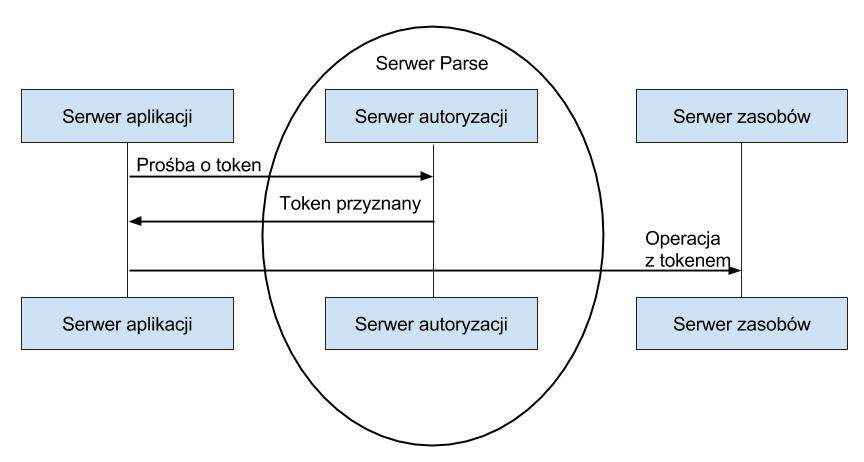
\includegraphics[width=12cm]{imgs/ch6_token.jpg}
    \caption
{Schemat działania JWT.}
    \label{fig:token}
\end{figure} 

Victor Albertos zdecydował się użyć wyżej wymienionego rozwiązania, aby zwiększyć pielęgnowalność swojej aplikacji: móc modyfikować logikę biznesową nie modyfikując oprogramowania po stronie klienta. Serwer \textit{Parse}, jako rozwiązanie uniwersalne, zapewniał takie podejście i~wpisywał się doskonale w~koncepcję autora \textit{JSON Web Token Authentication for Android}.

\section{Zasada działania}
Użytkownik loguje się z~urządzenia z~zainstalowanym systemem Android za pomocą swojej nazwy użytkownika i~hasła do serwera \textit{Parse}. Jeżeli nie posiada jeszcze konta na serwerze, może założyć je bezpośrednio z~używanego programu. Jeżeli użytkownik istnieje, od chwili zalogowania może korzystać z~dostępnych mu usług serwera, a~logując się z~wielu urządzeń korzysta z~wielosesyjności systemu.  Użytkownik może również akualizować swoje dane na serwerze.

%\section{Analiza aplikacji pod względem testowalności}
%\label{analiza testowalnosci}
%W tej pracy autor skupia się na budowie aplikacji tylko z~punktu widzenia testowania aplikacji, nie będzie więc analizowany szczegółowo kod źródłowy programu. Przeprowadzone natomiast zostaną testy, na podstawie których można w~wystarczającej części ocenić, czy zmiana struktury oprogramowania na \textit{Clean Architecture} oraz zastosowanie  \textit{Test Driven Development} wpłynie pozytywnie na testowalność oprogramowania, w~tym przypadku tej wybranej aplikacji.

\subsection{Budowa analizowanej aplikacji w~wersji pierwotnej}
Schemat budowy aplikacji \textit{JSON Web Token Authentication for Android} w~wersji pierwotnej przedstawia rysunek \ref{fig:app_std}.

\begin{figure}[!htb]
    \centering
    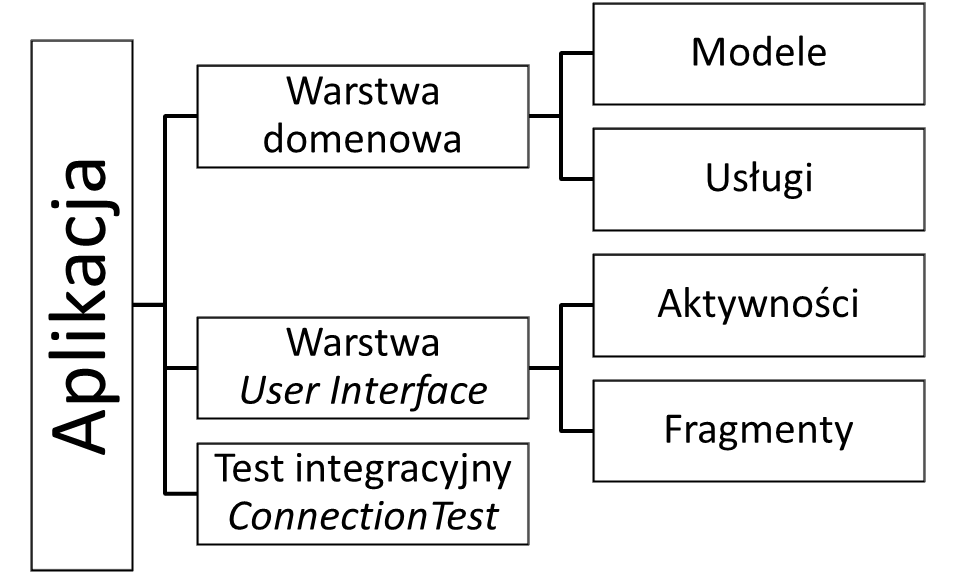
\includegraphics[width=8cm]{imgs/ch6_app_st_diagram.png}
    \caption
{Schemat budowy badanej aplikacji wykorzystującej architekturę standardową}
    \label{fig:app_std}
\end{figure} 

Aplikacja podzielona jest na moduł domeny i~moduł interfejsu użytkownika. W~celu przetestowania aplikacji, utworzono jeden test całkowicie zależny od środowiska Android, który w~zależności od kontekstu można nazwać integracyjnym, systemowym, bądź nawet końcowym. Dla potrzeb pracy traktowany jest jako test integracyjny, gdyż interesuje autora tylko wynik weryfikacji połączenia, bez zwracania uwagi na aspekty graficzne czy użytkowe związane z~docelowym urządzeniem. Test polega na zalogowaniu się do programu za pomocą przykładowych danych i~otrzymaniu wyniku, czy weryfikacja przebiegła pomyślnie. Poza tym przypadkiem nie stwierdzono żadnych innych testów, w~tym jednostkowych.

\subsection{Budowa analizowanej aplikacji w~wersji poprawionej}
Każde z~wymienionych w~rozdziale \ref{propozycja_rozwiazania} podejść do uporządkowania architektury systemowej można wykorzystać do polepszenia testowalności aplikacji tworzonych dla systemu Android. W~tym przypadku autor \textit{JSON Web Token Authentication for Android} zdecydował się na \textit{The Clean Architecture}, zaprezentowaną w~tej pracy w~rozdziale \ref{clean_architecture_opis}.

\newpage
Aplikacja w~wersji poprawionej nadal ma budowę modułową - tym razem moduły są trzy: moduł domeny, moduł danych i~moduł prezentacyjny. Zgodnie z~podejściem \textit{The Clean Architecture}, można rozpoznać poszczególne warstwy uporządkowanej architektury (rysunek \ref{fig:app_cl}):
\begin{figure}[!htb]
    \centering
    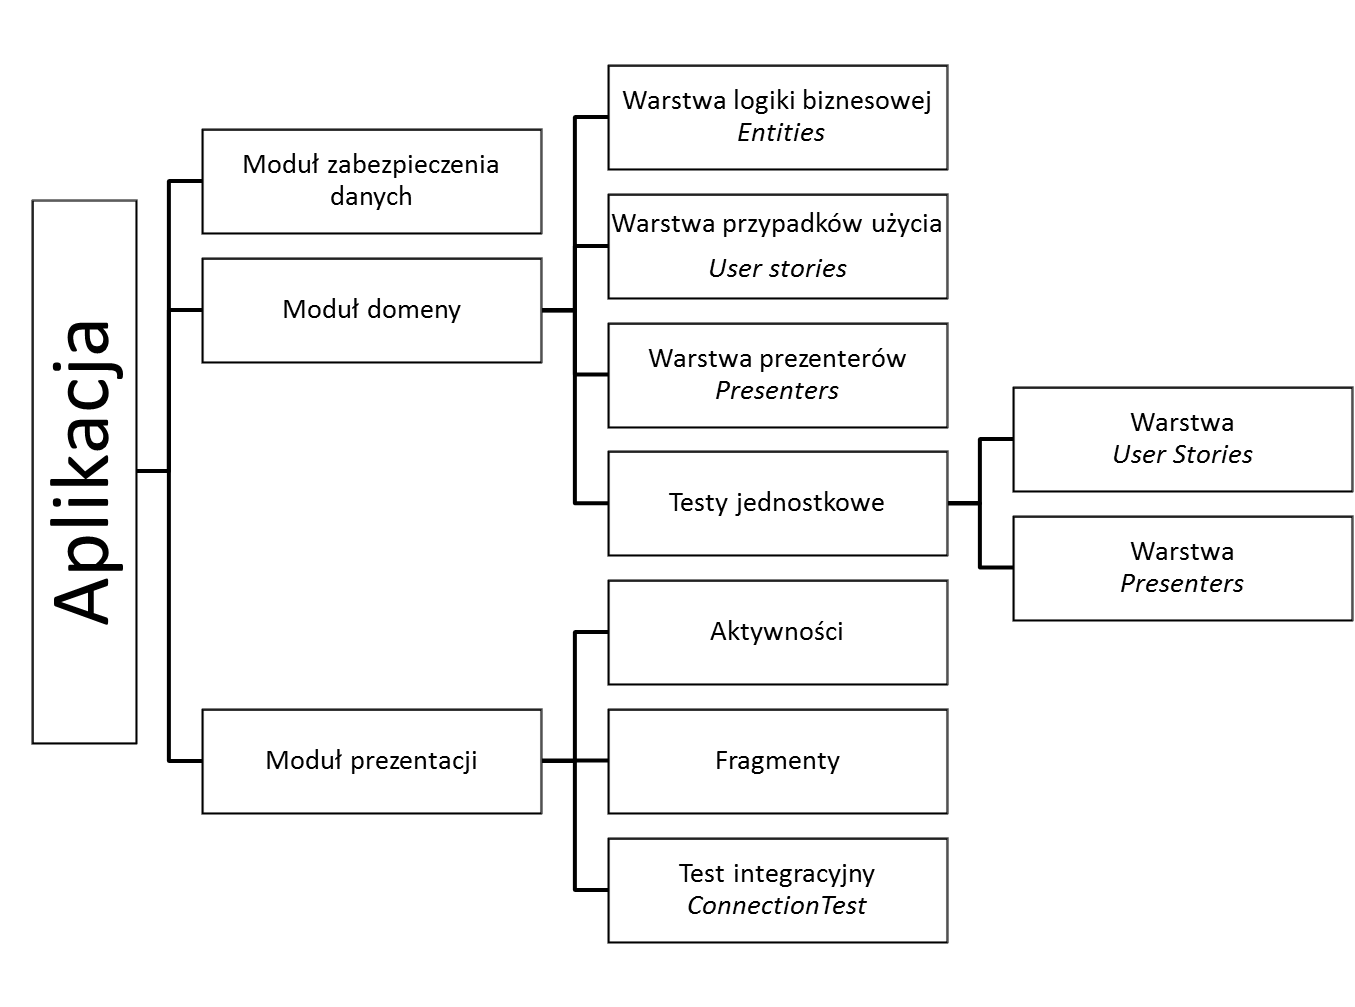
\includegraphics[width=12cm]{imgs/ch6_app_cl_diagram.png}
    \caption
{Schemat budowy aplikacji w~wersji poprawionej: warstwa \textit{entities}.}
    \label{fig:app_cl}
\end{figure} 

\begin{itemize}
\item
Warstwę \textit{entities}, w~której znajduje się definicja klasy \textit{User} oraz klasy \textit{Credentials}. Należą one do logiki biznesowej aplikacji i~to na tych klasach oparte jest działanie programu; 

\item
Warstwę \textit{Use Cases}, należącą do modułu domeny, do której na podstawie przypadków użycia zostały napisane testy jednostkowe;

\item
Warstwę \textit{Presenters}, również należącą do modułu domenowego i~odpowiadające jej testy jednostkowe; 

\item
Moduły \textit{data} oraz \textit{presentation}, to najbardziej zewnętrzna warstwa, zależna od wszystkich wyżej opisanych. 
\end{itemize}

Zgodnie z~ideą uporządkowanej architektury, warstwa \textit{entities} nie posiada informacji o~warstwach \textit{use cases}, przypadki użytkownika nie wiedzą nic o~warstwie prezentacyjnej, a~ta nie ma danych na temat warstw zewnętrznych, takich jak wspomniane bazy danych. Kierunek wstrzykiwania zależności jest zawsze od warstwy zewnętrznej do warstwy wewnętrznej.

\section{Przebieg doświadczenia}
Podczas doświadczenia wykonano zaprojektowane przez autora aplikacji testy dla obu wersji programu, wykorzystując to samo środowisko testowe\footnote{Środowisko testowe (ang. test environment) - środowisko, w~skład którego wchodzi sprzęt, wyposażenie, symulatory, oprogramowanie oraz inne elementy wspierające, potrzebne do wykonania testu. [wg IEEE 610]}: Android Studio w~wersji 1.5.1, ten sam sprzęt komputerowy i~ten sam emulator: Nexus\_5\_API\_23.

\section{Wyniki doświadczenia}
\label{wyniki_doswiadczenia}
\subsection{Wyniki dla testów jednostkowych}
W przypadku aplikacji w~wersji poprawionej testy jednostkowe istnieją dla warstw \textit{use cases} oraz \textit{presenters} Rezultat wykonania przedstawiają tabele \ref{tab:testy_jednostkowe_razem}, \ref{tab:testy_jednostkowe_usecases} i~\ref{tab:testy_jednostkowe_presenters}.
\begin{table}[!htb]
\centering
\caption{Zestawienie testów jednostkowych: podsumowanie dla warstw \textit{Use Cases} oraz \textit{Presenters}.}
\label{tab:testy_jednostkowe_razem}
\begin{tabular}{|p{5.8cm}|p{3cm}|p{3cm}|p{3cm}|}
\hline
\textbf{Warstwa} & \textbf{Przetestowane klasy} & \textbf{Przetestowane funkcje} & \textbf{Pokrycie linii kodu} \\ \hline
\textit{Use Cases} & 100\% (6/6) & 100\% (16/16) & 100\% (36/36)	\\ \hline
\textit{Presenters} & 100\% (15/15)	& 81\% (35/43) & 85\% (85/99) \\ \hline
\end{tabular}
\end{table}

\begin{table}[!htb]
\centering
\caption{Zestawienie testów jednostkowych: podsumowanie szczegółowe dla warstwy \textit{Use Cases}.}
\label{tab:testy_jednostkowe_usecases}
\begin{tabular}{|p{5.8cm}|p{3cm}|p{3cm}|p{3cm}|}
\hline
\textbf{Warstwa} & \textbf{Przetestowane klasy} & \textbf{Przetestowane funkcje} & \textbf{Pokrycie linii kodu} \\ \hline
\textit{GetUserUseCase} & 100\% (1/1) & 100\% (2/2) & 100\% (3/3)	\\ \hline
\textit{LoginUseCase} & 100\% (1/1) & 100\% (3/3) & 100\% (6/6)	\\ \hline
\textit{LogoutUseCase} & 100\% (1/1) & 100\% (2/2) & 100\% (3/3)	\\ \hline
\textit{SessionUseCase} & 100\% (1/1) & 100\% (3/3) & 100\% (14/14)	\\ \hline
\textit{SignUpUseCase} & 100\% (1/1) & 100\% (3/3) & 100\% (5/5)	\\ \hline
\textit{UpdateUserCase} & 100\% (1/1) & 100\% (3/3) & 100\% (5/5)	\\ \hline
\end{tabular}
\end{table}

\begin{table}[!htb]
\centering
\caption{Zestawienie testów jednostkowych: podsumowanie szczegółowe dla warstwy \textit{Presenters}.}
\label{tab:testy_jednostkowe_presenters}
\begin{tabular}{|p{5.8cm}|p{3cm}|p{3cm}|p{3cm}|}
\hline
\textbf{Warstwa} & \textbf{Przetestowane klasy} & \textbf{Przetestowane funkcje} & \textbf{Pokrycie linii kodu} \\ \hline
\textit{subscribers} & 100\% (3/3) & 80\% (8/10) & 91\% (22/24)	\\ \hline
\textit{GetUserPresenter} & 100\% (2/2) & 80\% (4/5) & 81\% (9/11)	\\ \hline
\textit{LaunchPresenter} & 100\% (2/2) & 83\% (5/6) & 85\% (12/14)	\\ \hline
\textit{LoginPresenter} & 100\% (2/2) & 80\% (4/5) & 81\% (9/11)	\\ \hline
\textit{LogoutPresenter} & 100\% (2/2) & 83\% (5/6) & 85\% (12/14)	\\ \hline
\textit{SignUpPresenter} & 100\% (2/2) & 80\% (4/5) & 81\% (9/11)	\\ \hline
\textit{UpdateUserPresenter} & 100\% (2/2) & 83\% (5/6) & 85\% (12/14)	\\ \hline
\end{tabular}
\end{table}

%\begin{figure}[!htb]
%    \centering
%    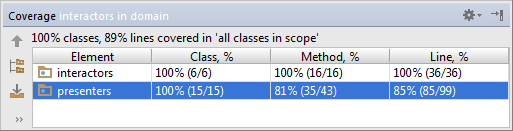
\includegraphics[width=12cm]{imgs/ch6_app_cl_test5.png}
%    \caption
%{Wyniki wraz z~pokryciem kodu}
%    \label{fig:app_cl_test5}
%\end{figure} 
%
%\begin{figure}[!htb]
%    \centering
%    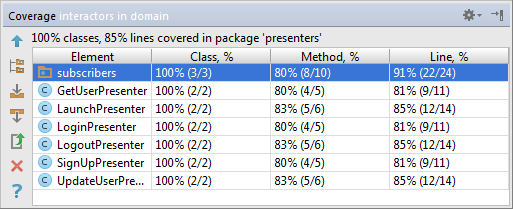
\includegraphics[width=12cm]{imgs/ch6_app_cl_test3.png}
%    \caption
%{Wyniki wraz z~pokryciem kodu}
%    \label{fig:app_cl_test3}
%\end{figure} 
%
%\begin{figure}[!htb]
%    \centering
%    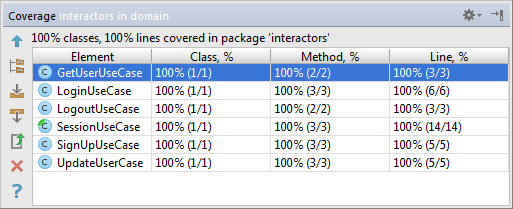
\includegraphics[width=12cm]{imgs/ch6_app_cl_test4.png}
%    \caption
%{Wyniki wraz z~pokryciem kodu}
%    \label{fig:app_cl_test4}
%\end{figure} 

W aplikacji w~wersji pierwotnej nie zaprojektowano testów jednostkowych w~ogóle, a~testując funkcjonalność programu zdano się w~całości na automatyczny test integracyjny. 

\newpage
W przypadku aplikacji w~wersji poprawionej, jak przedstawiają tabele \ref{tab:testy_jednostkowe_usecases} i~\ref{tab:testy_jednostkowe_presenters}, zaprojektowano 6 testów opartych na przypadkach użycia oraz 7 testów dla prezenterów, czyli łącznie 13 testów jednostkowych (równanie \ref{eq:test3}).
\begin{equation}
6+7 = 13 \label{eq:test3}
\end{equation}
W~przypadku aplikacji w~wersji pierwotnej - zgodnie z~wyjaśnieniem, które autor umieścił w~rozdziale \ref{testowanie_starej_struktury} - aby pokryć ten sam obszar funkcjonalności należałoby zaprojektować 42 testy jednostkowe (równanie \ref{eq:test4}).
\begin{equation}
6*7 = 42 \label{eq:test4}
\end{equation}
Różnicę tę uwidoczniono na wykresie \ref{fig:app_ut_liczba}.
\begin{figure}[!htb]
    \centering
    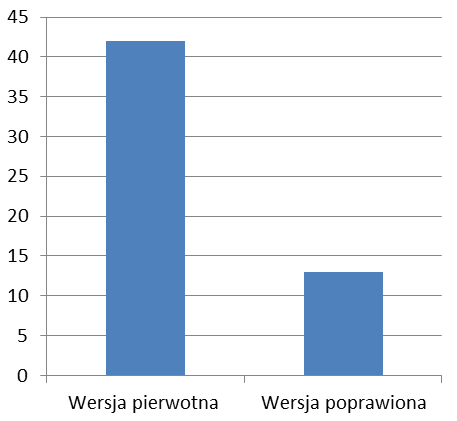
\includegraphics[width=8cm]{imgs/ch6_app_ut_liczba.png}
    \caption
{Porównanie ilości testów jednostkowych potrzebnych do pokrycia tej samej funkcjonalności w~przypadku wersji pierwotnej i~poprawionej. }
    \label{fig:app_ut_liczba}
\end{figure} 

Taka liczba testów musiała się również wpłynąć na ich czas wykonania, co w~przypadku badanej aplikacji przedstawia wykres \ref{fig:app_ut_czas}:
\begin{figure}[!htb]
    \centering
    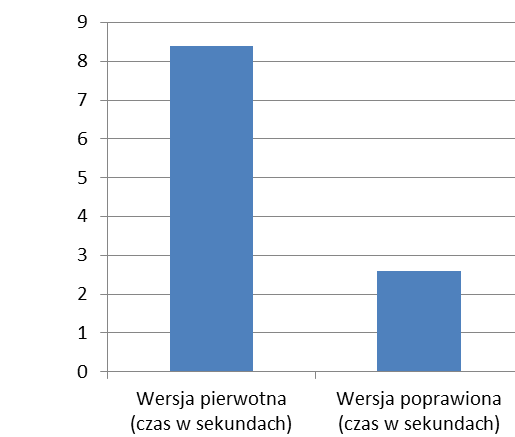
\includegraphics[width=8cm]{imgs/ch6_app_ut_czas.png}
    \caption
{Porównanie czasu wykonania testów jednostkowych potrzebnych do pokrycia tej samej funkcjonalności w~przypadku wersji pierwotnej i~poprawionej. }
    \label{fig:app_ut_czas}
\end{figure} 

\subsection{Testy integracyjne}
Dla obu opisywanych wersji zaprojektowano test integracyjny \textit{ConnectionTest}, dla którego przewidziano taki sam zakres testowania: generowany jest zestaw kilku użytkowników dla których przeprowadzano próbę połączenia. Czas trwania całego testu od uruchomienia do otrzymania wyniku pozytywnego bądź negatywnego (wraz z~uruchomieniem emulatora systemu Android w~wybranym do badań środowisku testowym) wyliczony w~doświadczeniu wyniósł około 200 sekund. 

W przypadku gdy dla aplikacji w~wersji pierwszej nie stwierdzono testów jednostkowych, to:
\begin{itemize}
\item
zakładając, że każdy z~sześciu testów jednostkowych opartych na przypadkach użycia dla aplikacji w~wersji poprawionej znalazłby jeden błąd, liczba powtórzeń testu \textit{ConnectionTest} w~najgorszym razie mogłaby wzrosnąć sześciokrotnie;
\item
zakładając, że dodatkowo każdy z~siedmiu testów jednostkowych przeznaczonych dla prezenterów również znalazłby błąd, ilość powtórzeń testu \textit{ConnectionTest} w~najgorszym przypadku mogłaby wzrosnąć 42-krotnie do momentu uzyskania wyniku pozytywnego (zostało to zaprezentowane na wykresie \ref{fig:app_int_czas}).
\end{itemize}
\begin{figure}[!htb]
    \centering
    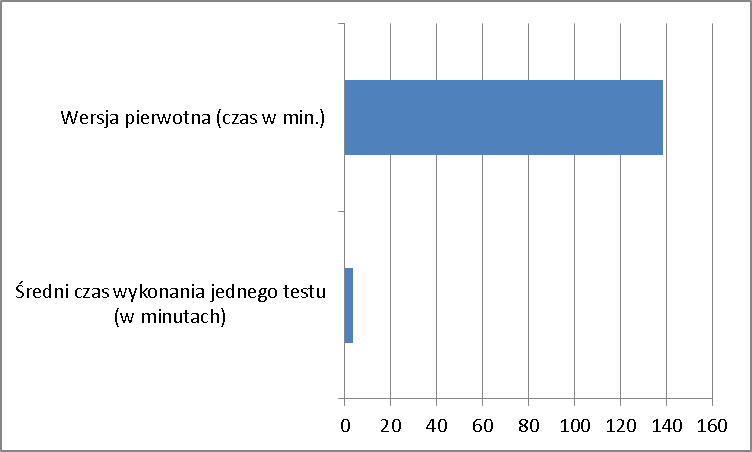
\includegraphics[width=8cm]{imgs/ch6_app_int_czas.png}
    \caption
{Porównanie czasu wykonania testów integracyjnych potrzebnych do pokrycia tej samej funkcjonalności w~przypadku wersji pierwotnej i~poprawionej. }
    \label{fig:app_int_czas}
\end{figure} 

\newpage
\section{Wnioski końcowe}
Powyższe doświadczenie pokazuje, że wykorzystanie architektury \textit{Clean Architecture} oraz podejścia \textit{Test Driven Development} wydaje się właściwe dla polepszenia testowalności badanej aplikacji zarówno w~przypadku, gdy w~wersji pierwotnej nie napisano w~ogóle testów jednostkowych, jak i~gdyby je zaprojektowano dla takiego samego obszaru testowania, co w~przypadku programu w~wersji poprawionej. Korzyści z~zastosowania danych rozwiązań pokazują wykresy \ref{fig:app_ut_liczba} i~\ref{fig:app_ut_czas}.

Udowodniono, że nawet jeżeli testy jednostkowe w~aplikacji pierwotnej zostałyby napisane, do przetestowania tego samego obszaru funkcjonalności ich liczba musiałaby być zdecydowanie większa od liczby ich odpowiedników w~przypadku aplikacji poprawionej. Wymagałoby to odpowiednio większego nakładu pracy pielęgnacyjnej przy ewentualnej modyfikacji programu. Zmiana kodu programu w~zakresie rozszerzenia funkcjonalności również wymagałaby napisania większej ilości dodatkowych testów jednostkowych.

Gdyby testów jednostkowych, tak jak w~badanym przypadku aplikacji w~wersji pierwotnej nie było, wtedy potrzeba zwiększenia czasu przeznaczonego na testy integracyjne i~wyższego szczebla jest jeszcze większa, co przedstawia wykres \ref{fig:app_int_czas}.

Przeprowadzone doświadczenie dowodzi, że warto wykorzystać opisywane w~rozdziale \ref{propozycja_rozwiazania} metody do zwiększenia testowalności, a~także - jak się okazuje - pielęgnowalności aplikacji przeznaczonych dla systemu Android. 